\section{Use case: Dental images}

An use case for this panoramics is dental health images. In this context, X-ray images could have hidden teeth by other ones, as shown in Fig. \ref{fig:dental_problem}.

\begin{figure}[H]
    \centering
    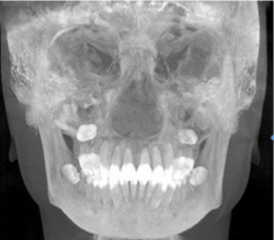
\includegraphics{img/dental_problem.png}
    \caption{Some teeth are hidden}
    \label{fig:dental_problem}
\end{figure}

Yun \textit{et al.} \cite{yun_automatic_2019} came up with a solution for this problem using panoramic images. Their proposal is shown in Fig. \ref{fig:proposal}.

\begin{figure}[H]
    \centering
    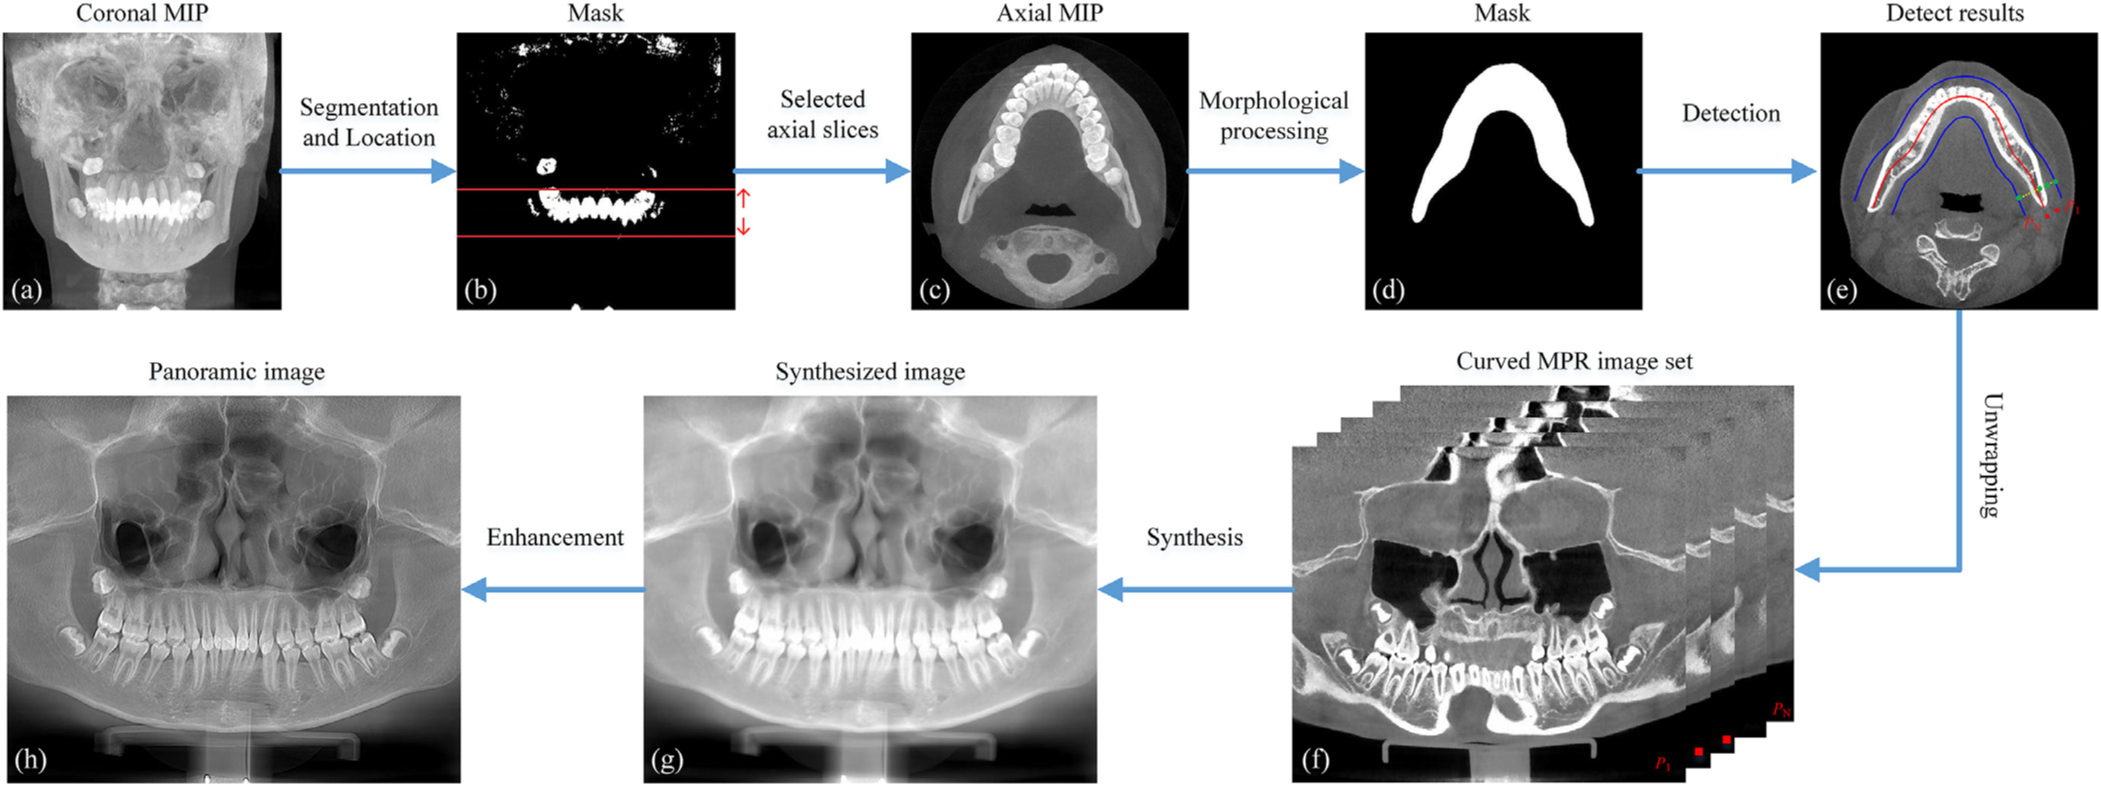
\includegraphics[width=0.9\textwidth]{img/dental_proposal.png}
    \caption{Proposed methodology}
    \label{fig:proposal}
\end{figure}

Firstly, they use thresholding based on the histogram of the image to build an accurate mask of the whole teething. After that, they estimate the dental arch using the following approximation:
\begin{gather*}
    I_0(i, j) = S \cdot \log \left( \sum_{n=1}^N e^{\frac{P_n(i,j)}{S}} \right)
\end{gather*}

This arch approximation can be used together with a lot of images around the whole head, and homographies to create an unwrapped version of the teething (Fig. \ref{fig:dental_pano}).

\begin{figure}[H]
    \centering
    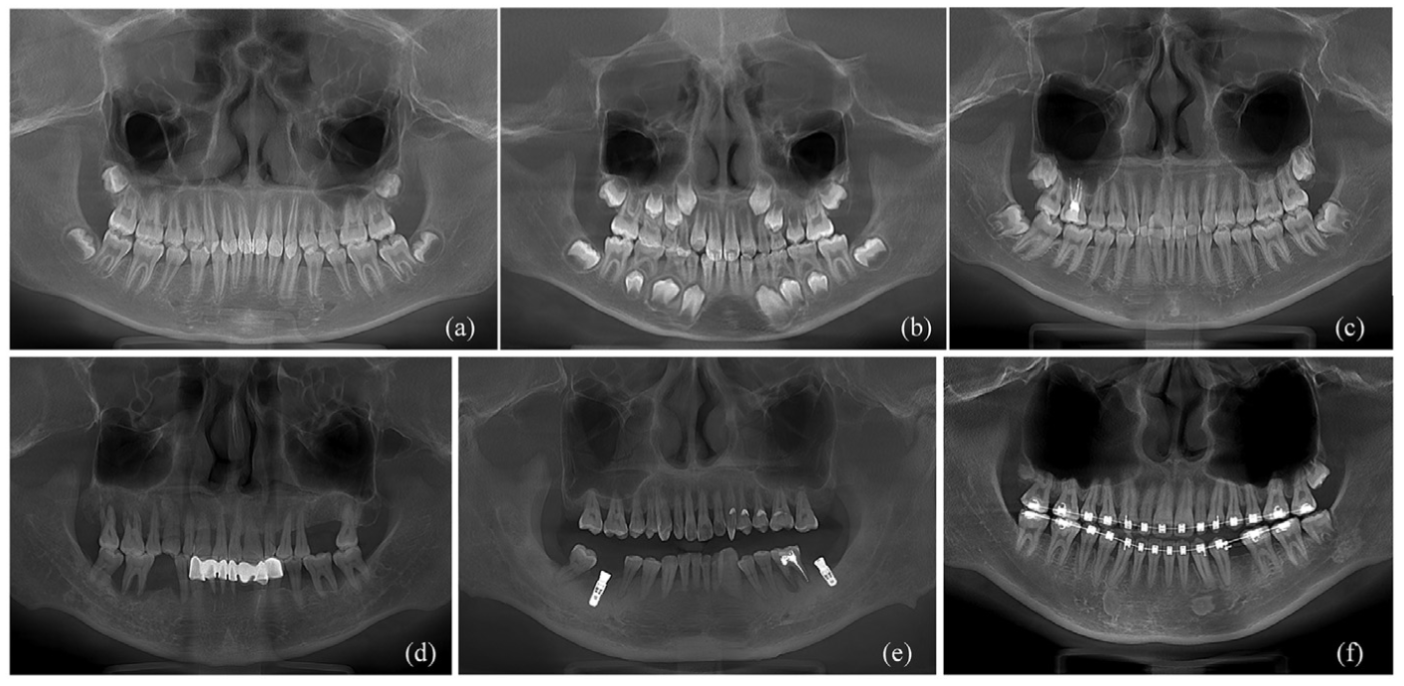
\includegraphics[width=0.6\textwidth]{img/dental_pano.png}
    \caption{Unwrapped images}
    \label{fig:dental_pano}
\end{figure}
